%! TEX root = diffusr.tex

\section{Appendix}\label{sec:appendix}

\subsection{Missing Proofs}\label{sec:missingproofs}

\begin{proof}[Proof of \cref{lem:wrongsampling}]
  Let $\odataset = \{ \{1, 2\}, \{1, 3\}, \{3\} \}$, and assume, w.l.o.g., that
  $\odataset'$ is the seq-dataset $\dataset'$ from~\eqref{eq:sampledataset},
  then clearly the matrix $M_{\dataset'}$ from~\eqref{eq:sampledatasetmatrix}
  belongs to $\matrices$.

  The set $\matrices$ also contains the matrix $M''$ obtained by swapping the
  first two rows of $M_{\dataset'}$ from~\eqref{eq:sampledatasetmatrix}, which
  corresponds to the seq-dataset $\dataset'' = \langle \{1, 3\}, \{1, 2\}, \{3\}
  \rangle$. The seq-datasets $\dataset'$ from~\eqref{eq:sampledataset} and
  $\dataset''$ are \emph{different}, but their corresponding datasets
  respectively are \emph{the same dataset}, i.e., $\mattodat{M_{\dataset'}} =
  \mattodat{M''}$. Thus, the set $\matrices$ contains \emph{at least two}
  matrices mapped to seq-datasets that, when seen as bags, are equal to
  $\odataset$. From the definition of $\matrices$, it holds that $\matrices$
  also contains
  \[
    A \doteq \left[
    \begin{array}{ccc}
      1 & 0 & 1 \\
      1 & 0 & 1 \\
      0 & 1 & 0
    \end{array}
    \right] \enspace.
  \]
  It holds that $\mattodat{A} = \{\{1,3\}, \{1, 3\}, \{2\}\}$. Again from the
  definition of $\matrices$, it holds that there is no other matrix $B$
  different than $A$ in $\matrices$ such that $\mattodat{B}= \mattodat{A}$.
  Thus, if we sample a matrix $M$ uniformly at random from $\matrices$ there is
  a higher probability that $\mattodat{M} = \odataset$ than $\mattodat{M} =
  \mattodat{A}$, and our proof is complete.
\end{proof}

\begin{proof}[Proof of \cref{lem:numcopies}]
  Recall that $\matrices$ depends on the observed dataset $\odataset$ and on the
  arbitrary ordering of its transactions chosen by \gioalgo, as the ordering
  fixes the row-sums $\rowsum{i}$, $1 \le i \le \rowsnum$ of the matrices in
  $\matrices$. In other words, it fixes the row indices of rows corresponding to
  transactions of length $\ell_i$, $1 \le i \le z_\dataset$, of
  $\dataset$. Thus, the number of different ways in which the transactions of
  $\dataset$ can be assigned to the rows of a matrix in $\matrices$ is the
  product, over the lengths in $L_\dataset$, of the number $q_i$ of different
  ways in which the transactions in $T_i$ can be assigned, i.e.,
  \[
    \copiesnum{\dataset} = \prod_{i=1}^{z_\dataset} q_i \enspace.
  \]
  Thus, we only have to argue that
  \[
    q_i = \binom{\card{T_i}}{\card{W_{i,1}}, \dotsc,
    \card{W_{i,h_i}}},
  \]
  which is true because the multinomial coefficient $\binom{n}{k_1,\dotsc,k_h}$
  is the number of different permutations of a bag containing $n$ objects such
  that $k_1$ objects are indistinguishable among themselves and of type 1, $k_2$
  objects are indistinguishable among themselves and of type 2, and so
  on~\citep[Eq.~1.22]{Stanley11}.
\end{proof}

\begin{proof}[Proof of \cref{thm:correctnaive}]
 A dataset $\dataset  \in \nullset$ is returned in output by \naivealgo\ iff a
 matrix $M$ such that $\mattodat{M} = \dataset$ is sampled. There are
 $\copiesnum{\dataset}$ such matrices $M$, each with a probability
 $\samplprob(M)$ as in~\eqref{eq:naivestatprob} to be sampled, from the
 properties of MCMC sampling with MH\@. Thus, the probability of returning
 $\dataset$ is exactly $\nullprob(\dataset$).
\end{proof}

\begin{proof}[Proof of \cref{lem:spairsnum}]
  We start by showing that, independently from the value of
  $\spairsfactor(t_a,t_b)$, all the swaps from $\dataset'$ to $\dataset''$ must
  involve transactions that are identical to $t_a$ and $t_b$, i.e, be in the
  form $((t_a,x),(t_b,y))$, for some $x,y\in \items$. Let $((t_c,c), (t_d,d))$
  be a swap from $\dataset'$ to $\dataset''$. We want to show that $((t_c,c),
  (t_d,d)) = ((t_a,a),(t_b,b))$.  Let $\bar{t}_a = (t_a \setminus \{a\}) \cup
  \{b\}$, $\bar{t}_b = (t_b \setminus \{b\}) \cup \{a\}$, $\bar{t}_c = (t_c
  \setminus \{c\}) \cup \{d\}$, and $\bar{t}_d = (t_d \setminus \{d\}) \cup
  \{c\}$. Then,
  \[
    (\dataset' \setminus \{ t_a, t_b \}) \cup \{ \bar{t}_a, \bar{t}_b \} =
    (\dataset' \setminus \{ t_c, t_d \}) \cup \{ \bar{t}_c, \bar{t}_d \}
  \]
  since both sides are equal to $\dataset''$. Since datasets are \emph{bags}, the
  operations of difference and union are effectively one the inverse of the
  other. Thus, we can write
  \[
    \dataset' \cup \{ \bar{t}_a, \bar{t}_b \} \cup \{ t_c, t_d \} = \dataset'
    \cup \{ \bar{t}_c, \bar{t}_d \} \cup \{ t_a, t_b \} \enspace.
  \]
  We can remove $\dataset'$ from both sides to get
  \begin{equation}\label{eq:spairsnumtech}
    \{ \bar{t}_a, \bar{t}_b, t_c, t_d \} = \{ \bar{t}_c, \bar{t}_d, t_a, t_b \}
    \enspace.
  \end{equation}
  By definition of a swap, it must be $t_a \neq \bar{t}_a$ and $t_a \neq
  \bar{t}_b$, thus it must be either $t_a = t_c$ or $t_a = t_d$, and similarly
  for $t_b$.

  Assume now that $\card{t_a} \neq \card{t_b}$, then only one between $t_a =
  t_c$ and $t_a = t_d$ is actually possible so, w.l.o.g., let $t_a = t_c$ and
  $t_b = t_d$. Then from these facts and~\eqref{eq:spairsnumtech}, it must be
  $\{ \bar{t}_a, \bar{t}_b \} = \{ \bar{t}_c, \bar{t}_d \}$, thus either
  $\bar{t}_a = \bar{t}_c$ or $\bar{t}_a = \bar{t}_d$. Since $\card{\bar{t}_a} =
  \card{t_a} = \card{t_c} = \card{\bar{t}_c}$ and $\card{\bar{t}_d} =
  \card{t_d} = \card{t_b}$, then it can only be $\bar{t}_a = \bar{t}_c$, which
  implies $c = a$, and similarly it must be $b = d$. Thus, if $\card{t_a} \neq
  \card{t_b}$, then all swaps from $\dataset'$ to $\dataset''$ are equal to
  $((t_a,a), (t_b,b))$, which implies the thesis for this case.

  Assume now that $\card{t_a} = \card{t_b}$ but $\card{t_a \setminus t_b}$ and
  $\card{t_b \setminus t_a}$ are different than 2 (the two asymmetric set
  differences must have the same size, since the two sets have the same size).
  From the first part of the proof, we have that it must be either $t_a = t_c$
  or $t_a = t_d$, and similarly for $t_b$. W.l.o.g., let $t_a = t_c$ and $t_b =
  t_d$.  If $\card{t_a \setminus t_b} = \card{t_b \setminus t_a} = 1$, then $a$
  and $b$ are the only two items that can be swapped, so it must be $c = a$ and
  $b = d$. Thus, in this specific subcase, all swaps from $\dataset'$ to
  $\dataset''$ are equal to $((t_a,a), (t_b,b))$, which implies the thesis for
  this case. Assume now that $\card{t_a \setminus t_b} = \card{t_b \setminus
  t_a} > 2$.  From these facts and~\eqref{eq:spairsnumtech}, it must be $\{
  \bar{t}_a, \bar{t}_b \} = \{ \bar{t}_c, \bar{t}_d \}$, thus either $\bar{t}_a
  = \bar{t}_c$ or $\bar{t}_a = \bar{t}_d$. We now show that it must be
  $\bar{t}_a = \bar{t}_c$. Assume by contradiction that $\bar{t}_a = \bar{t}_d$.
  Since $t_c = t_a$, it holds $\bar{t}_a = t_c \setminus \{a\} \cup \{b\}$.
  Thus, it must be
  \[
    (t_c \setminus \{a\}) \cup \{b\} = (t_d \setminus \{d\}) \cup \{c\} \enspace.
  \]
  Since $a, c \in t_c$ and $b \notin t_c$, by taking the asymmetric set
  differences between each side of the above identity and $t_c$ we get
  \[
    \{ b \} = (t_d \setminus \{d \}) \setminus t_c
  \]
  which means that $t_d \setminus t_c  = t_b \setminus t_a = \{b, d\}$, i.e.,
  this set difference has size equal to 2, which is a contradiction since we
  assumed that $\card{t_b \setminus t_a} > 2$. Thus, it must be $\bar{t}_a =
  \bar{t}_c$, which implies $c = a$, and similarly it must be $b = d$. Thus, all
  swaps from $\dataset'$ to $\dataset''$ are equal to $((t_a,a), (t_b,b))$,
  which implies the thesis for this case.

  We have therefore shown that the thesis is true for the case
  $\spairsfactor(t_a,t_b)=1$. Consider now the other case, which means that
  $\card{t_a} = \card{t_b}$ and $\card{t_a \setminus t_b} = \card{t_b \setminus
  t_a} = 2$. W.l.o.g., let $t_a \setminus t_b = \{a, z\}$ and $t_b \setminus t_a
  = \{b, w\}$.  It is easy to see that the swaps $((t_a,a), (t_b,b))$ and
  $((t_a,z), (t_b,w))$ lead to the same dataset $\dataset''$, while the other
  two swaps $((t_a,a), (t_b,w))$ $((t_a,z), (t_b,b))$ lead to a different
  dataset. Thus, there are $\spairsfactor(t_a,t_b)=2$ swaps from $\dataset'$ to
  $\dataset''$ involving the transactions $t_a$ and $t_b$. From the first part
  of the proof, we have that all swaps from $\dataset'$ to $\dataset''$ must
  involve transactions identical to $t_a$ and $t_b$, hence we obtain the thesis
  for this case.
\end{proof}

\begin{proof}[Proof of \cref{thm:totspairsnumdat}]
  Let $((t_a, a), (t_b, b))$ be any of the $\totspairsnummat{M_\dataset}$
  swaps from $M_\dataset$ to any $M$ of its neighbor matrices in the Markov
  chain used by \gioalgo. From the definitions of ``swap'' for \gioalgo\ and for
  \refalgo, it follows that $((t_a, a), (t_b, b))$ is a valid swap for
  $\refalgo$ iff $\mattodat{M} \neq \dataset$, i.e., if the dataset
  corresponding to $M$ is not $\dataset$ itself. The number of valid
  swaps from $\dataset$ is therefore $\totspairsnummat{M_\dataset}$ minus the
  total number of swaps from $M_\dataset$ to any $M$ of its neighbors with
  $\mattodat{M} = \dataset$. We now show that the number of such
  ``self-swaps'' is $\selfspairsnum{\dataset}$.

  For a neighbor $M \neq M_\dataset$ of $M_\dataset$ to have $\mattodat{M} =
  \dataset$ it must be that that there is a swap $((t_a, a), (t_b, b))$ such
  that
  \[
    (t_a \setminus \{a\}) \cup \{b\} = t_b\ \text{and}\ (t_b \setminus \{b\})
    \cup \{a\}=t_a \enspace.
  \]
  Since $a \in t_a \setminus t_b$ and $b \in t_b \setminus t_a$, the above is
  possible iff $\card{t_a} = \card{t_b}$ and $\{a\} = t_a \setminus t_b$ and
  $\{b\} = t_b \setminus t_a$. The number of such \emph{unordered} pairs of
  transactions (i.e., the number of self-swaps) is as
  in~\eqref{eq:selfspairsnum}, where the factor $\sfrac{1}{2}$ is to correct for
  the fact that the considered set contains \emph{ordered} pairs of
  transactions.
\end{proof}

\begin{proof}[Proof of \cref{lem:sampleneighbor}]
  The procedure keeps sampling candidate swaps (i.e., pairs of elements of
  $\spairs$) until it finds one that is a valid swap. Since each element of
  $\spairs$ is sampled independently and uniformly at random from $\spairs$,
  then the candidate swap is chosen uniformly at random among all candidate
  swaps, thus, if it is valid, is also chosen uniformly at random among all
  valid swaps, i.e., each valid swap has a probability of
  $1/\totspairsnumdat{\dataset'}$ of being chosen among all valid swaps, as
  there is one and only one pair of elements of $\spairs$ for each valid swap.
  $\dataset''$ is output whenever the procedure chooses one of the
  $\spairsnum{\dataset'}{\dataset''}$ valid swaps leading to it from
  $\dataset'$. Thus, the probability of outputting $\dataset''$ is the sum of
  the probabilities of choosing each of these swaps, hence the thesis.
\end{proof}

\subsection{Computing $\copiesnum{\mattodat{M''}}$ from
  $\copiesnum{\mattodat{M'}}$}\label{sec:copiesnum}

Using the notation from the statement of \cref{lem:numcopies}, given a
transaction $t \in \mattodat{M'}$, suppose $t \in T_i$ for $1 \leq i \leq
z_{\mattodat{M'}}$. Further suppose $t = \tau_{i, j} \in \bar{T}_i$, where $1
\leq j \leq h_i$. Let $\mathsf{net}$ be a dictionary that maps each different
transaction $t \in \mattodat{M'}$ to $\card{W_{i, j}}$, i.e., the size of the
bag of transactions equal to $t$ (including $t$). This data structure is easy to
initialize and keep up to date. We can then obtain $\copiesnum{\mattodat{M'}}$
from $\copiesnum{\mattodat{M''}}$ as shown in \cref{algo:getcopiesnumneigh},
which leverages the fact that $\copiesnum{\mattodat{M'}} =
\copiesnum{\mattodat{M''}}$ if $\mattodat{M''} = \mattodat{M'}$
(\cref{algline:samedat}), and the definition of the multinomial to greatly
simplify the computation
(lines~\ref{algline:updatestart}--\ref{algline:updateend}).

\begin{algorithm}[ht]
  \caption{Computing $\copiesnum{\mattodat{M''}}$ from
  $\copiesnum{\mattodat{M'}}$}\label{algo:getcopiesnumneigh}
  \DontPrintSemicolon%

  \SetKwData{NumEqTransac}{net}

  \KwIn{Value $\copiesnum{\mattodat{M'}}$, valid swap $((t_a,a), (t_b,b))$ from
  $\mattodat{M'}$ to $\mattodat{M''}$, dictionary $\NumEqTransac$}

  \KwOut{$\copiesnum{\mattodat{M''}}$}

  $\bar{t}_a \gets (t_a \setminus \{a\}) \cup \{b\}$,  $\bar{t}_b \gets (t_b
  \setminus \{b\}) \cup \{a\}$\;

  \lIf{$t_a =
    \bar{t}_b$}{\Return{$\copiesnum{\mattodat{M'}}$}}\label{algline:samedat}

  \ForEach{$i \in \{a,b\}$}{\label{algline:updatestart}
    \leIf{\NumEqTransac\ has key $\bar{t}_i$}{$\beta_i \gets
      \NumEqTransac[\bar{t}_i]$}{$\beta_i \gets 0$}
  } % \ForEach{$i \in \{a,b\}$}{

  \Return{$\copiesnum{\mattodat{M'}} \frac{\NumEqTransac[t_a]
        \NumEqTransac[t_b]}{(\beta_a + 1) (\beta_b +
      1)}$}\label{algline:updateend}
\end{algorithm}

% 20220124 MR: commenting out as it doesn't seem to add much. We'll add it back
% in the journal version and in the thesis.
%\subsection{Sampling according to the refined neighborhood distribution
%$\neighprob_{\dataset'}(\dataset'')$}\label{sec:samplerefinedneighprob}
%
%\begin{algorithm}[hb]
%  \caption{Sampling according to the refined neighborhood distribution
%  $\neighprob_{\dataset'}(\dataset'')$}\label{algo:samplerefinedneighprob}
%  \DontPrintSemicolon%
%
%  \SetKwRepeat{Do}{do}{while}
%
%  \KwIn{bag $\spairs \doteq \{(t,i) \suchthat t \in \dataset, i \in t\}$}
%
%  \KwOut{valid swap $((t_a,a), (t_b,b))$ from $\dataset'$ to $\dataset''$}
%
%  \lDo{$(a \in t_b) \vee (b \in t_a) \vee (t_a \setminus \{a\} = t_b \setminus
%  \{b\})$}{
%    $(t_a,a), (t_b,b) \gets$ uniform independent samples from $\spairs$
%  } % \Do{$(a \in t_b) \vee (b \in t_a) \vee (t_a \setminus \{a\} = t_b \setminus \{b\})$}{
%
%  \Return{$((t_a,a), (t_b,b))$}
%\end{algorithm}

\subsection{Additional Figures}\label{sec:addarsd}
See \cref{fig:addarsd}.

\begin{figure}[hbt]
  \centering
  \begin{subfigure}{0.40\textwidth}
    \centering
    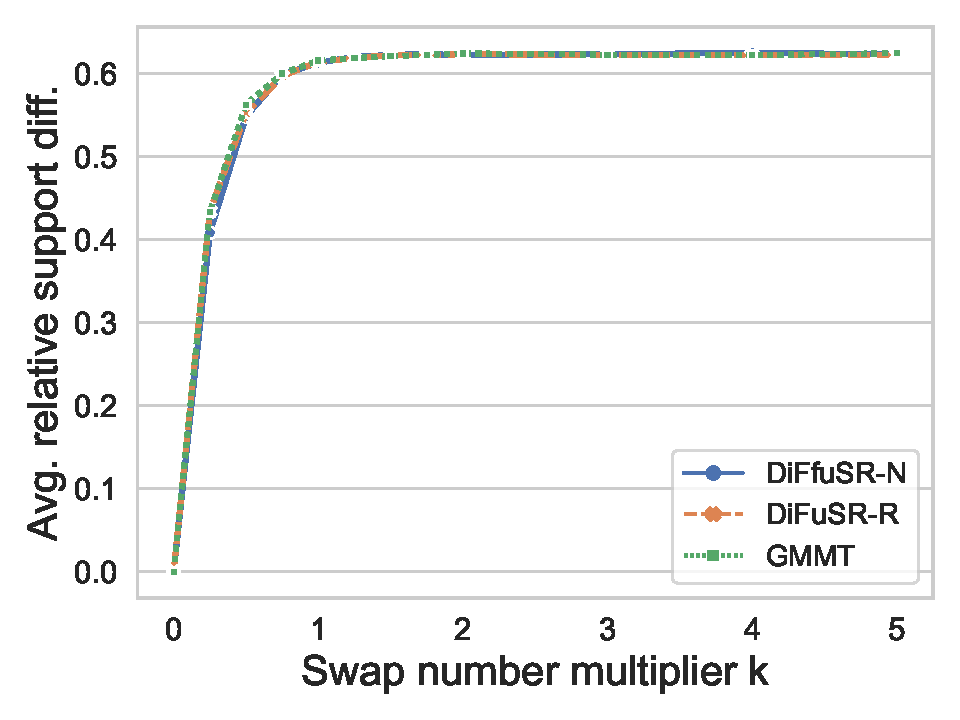
\includegraphics[width=\textwidth]{convergence-foodmart-5-0.0003-0.pdf} % chktex 8
    \caption{\textsc{Foodmart}}
  \end{subfigure}%

  \centering
  \begin{subfigure}{0.40\textwidth}
    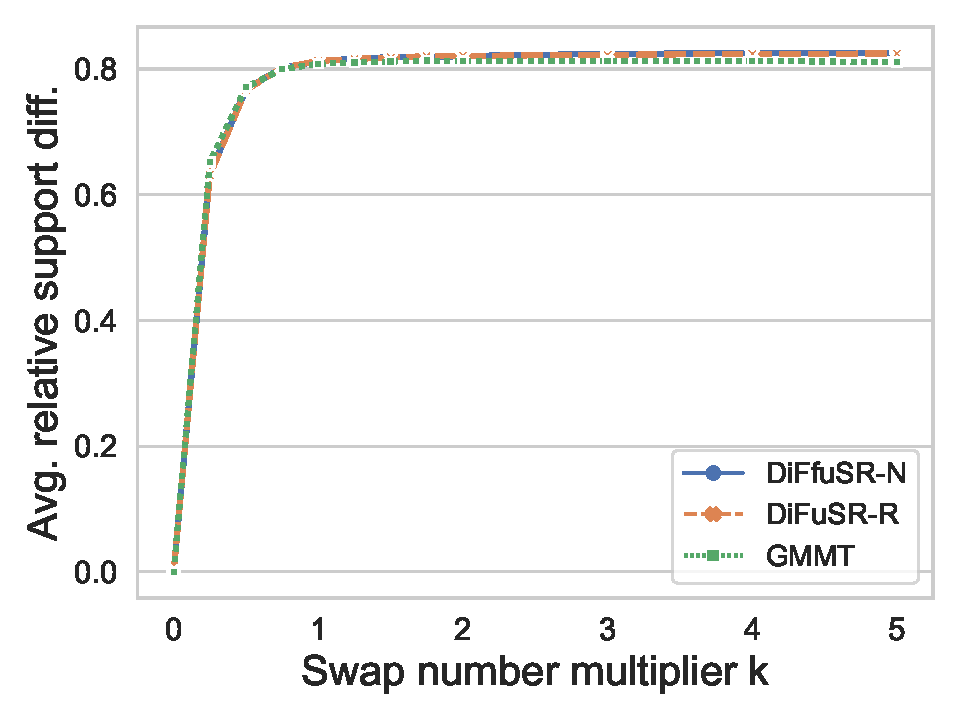
\includegraphics[width=\textwidth]{convergence-BMS2-5-0.002-0.pdf} % chktex 8
    \caption{\textsc{BMS 2}}
  \end{subfigure}
  \caption{Additional convergence results.}\label{fig:addarsd}
  \Description{Additional convergence results.}
\end{figure}
